\subsection{Reihen}
Eine Reihe ist eine Folge von Partialsummen und somit auch eine Abbildung von $\mathbb{N}$ nach $X$ (meist ist $X = \mathbb{R}$). Anders ausgedr"uckt, ist das $k$-te Reiheglied die Summe der ersten $k$ Folgenglieder einer Folge. Da Mathematiker schreibfaul sind und es sehr aufwendig ist ein Reihenglied hinzuschreiben da man $k$ Folgeglieder mit einen $+$ verknüpft aufschreiben m"usste, wurde ein neues, mathematisches Symbol eingef"uhrt, das so genannte "'Summen-Zeichen"' $\sum$.
%\vspace{1 cm}\\
%Folgende Grafik zeigt nun noch einmal aus welchen Teilen sich das Summen-Zeichen zusammen setzt:
%\vspace{0.5 cm}\\
\begin{minipage}{7 cm}
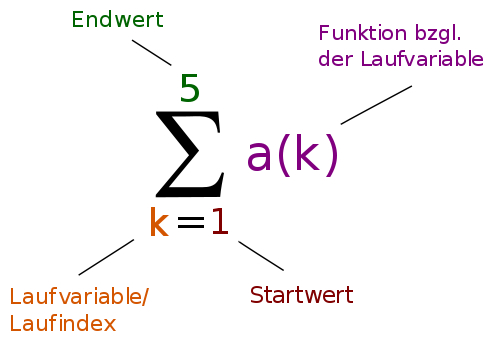
\includegraphics[width = 7 cm]{pictures/summe}
\begin{description}
\item[Endwert] Dieser Wert bestimmt, bis zu welchem Glied die Folge aufsummiert werden soll er kann auch unendlich $\infty$ sein.
\end{description}
\end{minipage}
\begin{minipage}{7 cm}
\begin{description}
\item[Startwert] Dieser Wert ist der erste Wert der Laufvariable und bestimmt somit das erste aufsummierte Folgeglied.
\item[Laufvariable] Diese Variable ist auch Teil des Bildungsgesetzes und wird pro aufsummierten Folgeglieds um 1 erh"oht, bis sie den Endwert erreicht hat.
\item[Funktion bzw. der Laufvariable] Hiermit ist das Bildungsgesetz der urspr"unglichen Folge gemeint.
\end{description}
\end{minipage}

\subsubsection{Endliche Reihen}
Als endliche Reihen werden Reihen bezeichnet, deren Startwert und Endwert nicht gegen Unendlich gehen. (Ich sage hier mit Absicht "'\textbf{gegen} plus oder minus Unendlich geht"', da der Wert Unendlich logischer Weise niemals erreicht werden kann, auch wenn Chuck Norris bis Unendlich z"ahlen kann...)

\subsubsection{Unendliche Reihen}
Was f"ur eine "Uberraschung, dass es bei Unendlichen Reihen nun so ist, dass der Endwert gegen Unendlich geht.
\begin{equation*}
s = \sum\limits_{k=0}^{\infty}g(k)
\end{equation*}

\subsubsection{Monotonie, Beschr"anktheit und Konvergenz}
Genau wie Folgen k"onnen auch Reihen monoton, beschr"ankt und konvergent gegen einen bestimmten Wert sein. Die Definition dieser Begriffe bleibt jedoch genau die selbe, wie auch bei Folgen, weshalb ich sie mir hier spare.

\subsection{Besondere Reihen}
\subsubsection{Konvergierende Reihen und Nullfolgen}
Das Bildungsgesetz jeder konvergierenden Reihe beschreibt eine Nullfolge.
\begin{center}
\textcolor{red}{Anders herum stimmt das allerdings nicht!}
\end{center}
Bekanntestes Gegenbeispiel hierf"ur ist die so genannte \textbf{Harmonische Reihe}:
\begin{equation*}
s_n = \sum\limits_{k=1}^{n}\frac{1}{k}
\end{equation*}
Diese Reihe divergiert gegen Unendlich! Sie wird auch als \textcolor{red}{harmonische Reihe} bezeichnet. Beweis mithilfe einer Absch"atzung:
\begin{align*}
s^{2^{k+}} &= 1 + \frac{1}{2} + \underbrace{\left( \frac{1}{3} + \frac{1}{4} \right)}_{\geq 2 \cdot \frac{1}{4}} + \underbrace{\left( \frac{1}{5} + \ldots + \frac{1}{8} \right)}_{\geq 4 \cdot \frac{1}{8}} + \ldots + \underbrace{\left( \frac{1}{2^k + 1} + \ldots + \frac{1}{2^{k+1}} \right)}_{\geq 2^k \cdot \frac{1}{2^{k + 1}}}\\
&\geq 1 + \frac{1}{2} + 2^{\color{red}1} \cdot \frac{1}{4} + 2^{\color{red}2} \cdot \frac{1}{8} + \ldots + 2^{\color{red}k} \cdot \frac{1}{2^{k+1}} \\
&= 1 + \frac{1}{2} + \underbrace{\frac{1}{2} + \frac{1}{2} + \frac{1}{2} + \ldots + \frac{1}{2}}_{k-\text{mal}}\\
&= 1 + \frac{1}{2} + \frac{1}{2} \cdot k =  1 + \frac{1}{2} + \frac{k}{2} = \frac{3 + k}{2}
\end{align*}

\subsubsection{Geometrische Reihen}
Jede geometrische Reihe kann auch wie folgt dargestellt werden:
\begin{equation*}
\sum\limits_{i=0}^{n} q^i = \begin{cases} \frac{1-q^{n+1}}{1-q} &\mbox{falls } q \neq 1 \\ 
n + 1 & \mbox{sonst.} \end{cases}
\end{equation*}
